%EXP

\subsection{Experimental Setup}

The 218 publicly-available and labeled patients were downloaded from NCBI and converted to FASTQ format using the SRA toolkit, and labeled according to the labels on EBI, as described in the Materials section. Each read was assembled with SOAPdenovo2, with the k-mer length set to 51, reads cut off after 100 base pairs (original length of 180 base pairs), and the average insert size set to 350 in accordance with the reported average insert size reported in the MGWAS study \cite{qin041012}. Assembly for each file took 7-30 minutes, depending on the file size, and each patient was assembled in parallel. Combining the files into one file took 12 minutes. Assembly was used for all of the classification methods tested, because the combining of individual reads and reduction in total data size made classification feasible.

\subsection{Methods Tested}

This section provides an overview of the different methods that we compared our pipeline to. Our pipeline uses clustering, whereas the other methods do not. Instead, those methods directly compare individual instances instead of clusters. In order to do this, sequence reads were represented as counts of k-mers. k-mers are nucleotide strings of length k. Since there are four possible nucleotides, the number of possible k-mers is \(4^k\). For instance, if k=3, there are \(4^3\) = 64 possible k-mers, which are AAA, AAC, AAG, AAT, ACA, ACC, ..., TTT. For a string "ATACGATA", the count for the k-mers is 2 for ATA, 1 for TAC, ACG, CGA, and GAT, and 0 for everything else. We wrote a script to represent the reads as vectors representing the k-mer counts in the string, and these vectors were used by the other methods. From experimental validation, we found a k-mer value of 3 to be the most effective.

\subsubsection{CAMIL: Our Pipeline}

We refer to our pipeline as "CAMIL", which stands for Clustering and Assembly with Multiple Instance Learning. We implemented two different versions of this pipeline: one that uses D-BoW feature extraction, and one that uses H-BoW feature extraction. These results are denoted as "CAMIL D-BoW" and "CAMIL H-BoW", respectively, in the results tables and graphs. Clustering for the pipeline with UCLUST took 10 hours and 51 minutes. Without the assembly step reducing the size of the data, clustering would not have been feasible. Feature extraction and SVM-light classification took 10 minutes and 17 seconds to run for D-BoW, versus 5 minutes and 14 seconds for H-BoW.

\subsubsection{MI-SVM and sbMIL}

MI-SVM \cite{andrews02} and sbMIL \cite{bunescu07} are two of the classic Multiple Instance Learning algorithms that fall into what Amores calls the "Instance Space" (IS) methods, in that they only use "local" information based on comparisons between individual instances and treat bag labels as aggregations of instance labels \cite{amores13}. Additionally, both of these methods follow the standard MIL assumption that bags with negative labels contain only negative instances, whereas positive bags contain one or more positive instances \cite{amores13}. sbMIL specifically assumes that positive bags contain few positive instances \cite{bunescu07}. We include these algorithms as an example of many of the early MIL algorithms, which usually fell into the IS paradigm and used the standard MIL assumption. For the implementation of these methods, we used an open-source Python implementation by Doran \cite{doran14}, which is available on GitHub\footnote{https://github.com/garydoranjr/misvm}.

\subsubsection{GICF}

The Group-Instance Cost Function (GICF) is a method proposed by Kotzias et al. that learns instance labels in addition to group labels \cite{kotzias15}. The cost function 

\subsubsection{Original MGWAS Paper: mRMR + SVM}

Temp

\subsection{Results For Bag/Patient Labels}

Temp

\subsection{Deriving Instance "Labels"}

\begin{figure}[t]
\centering
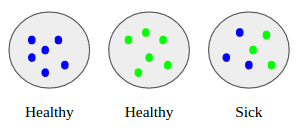
\includegraphics[scale=0.5]{./instance-labels.png}
\caption{This diagram illustrates why static instance labels are not sufficient for phenotype prediction. A patient with 6 of the blue microbe or 6 of the green microbe may be healthy, while a patient with 3 of each is sick. Static instance labels cannot capture this relationship. This is also explored by Amores in his MIL taxonomy \cite{amores13}.} \label{instance-labels}
\end{figure}

One of the benefits of using Multiple Instance Learning methods is that we can attempt to discover instance "labels". In fact, we did not attempt to apply static, unchanging labels to individual reads or clusters, since organisms are affected by their interactions with each other. For instance, a patient with X amount of microbe A or X amount of microbe B, but not with X/2 amount of microbe A and X/2 amount of microbe B. This is illustrated in Figure \ref{instance-labels}. This example is very simplified, but it explains why static instance labels are insufficient.

However, we can infer from the SVM decision boundary which clusters appear to be most relevant to the disease diagnosis. Since feature vectors are multiplied by the weight vector of the decision boundary to determine the label of the patient, we can assume that clusters with the highest weights in the weight vector are most relevant to the disease diagnosis. For instance, if the Ith scalar in the weight vector is has the highest value of any of the weights, then cluster I is likely to play a major role in the disease. Similarly, the most negative weights in the weight vector indicate clusters whose presence in a patient indicates that they likely do not have the disease. Because the data is metagenomic, the clusters represent both phylogenetic and functional similarity, so identifying the most relevant clusters can help discover more about the pathology of the disease. For Type 2 Diabetes, which is a complex phenotype and a disease that is both common and deadly, this is potentially quite valuable.